% DO NOT COMPILE THIS FILE DIRECTLY!
% This is included by the other .tex files.

\begin{frame}[t,plain]
\titlepage
\end{frame}

\begin{frame}
\frametitle{Objectives}
\begin{itemize}
        \item Learn how to use MISP to support common OSINT gathering use-cases often used by SOC, CSIRTs and CERTs
                \begin{itemize}
                        \item Use practical exercise examples\footnote{\url{https://gist.github.com/adulau/8c1de48060e259799d3397b83b0eec4f}}
                        \item The exercises are based on {\bf practical recent cases to model and structure intelligence} using the MISP standard
                \end{itemize}
        \item Improve the data models available in MISP by exchanging live improvements and ideas
        \item Be able to share the results to the community at the end of this session
\end{itemize}
\end{frame}

\begin{frame}
\frametitle{(Threat) Intelligence}
\begin{itemize}
        \item {\bf Cyber threat intelligence (CTI) is a vast concept} which includes different concepts, methods, and workflows
                \begin{itemize}
                        \item Intelligence is defined differently in the military than in the financial sector than in the intelligence community
                \end{itemize}
        \item {\bf MISP project doesn't want to lock an organisation or a user into a specific model}. Each model is useful depending on the objectives of an organisation
        \item A set of pre-defined knowledge base or data-models are available and organisations can select (or create) what they need
        \item During this session, an overview of the most used taxonomies, galaxies, and objects will be described
\end{itemize}
\end{frame}

\begin{frame}
        \frametitle{Overall process of collecting and analysing OSINT}
        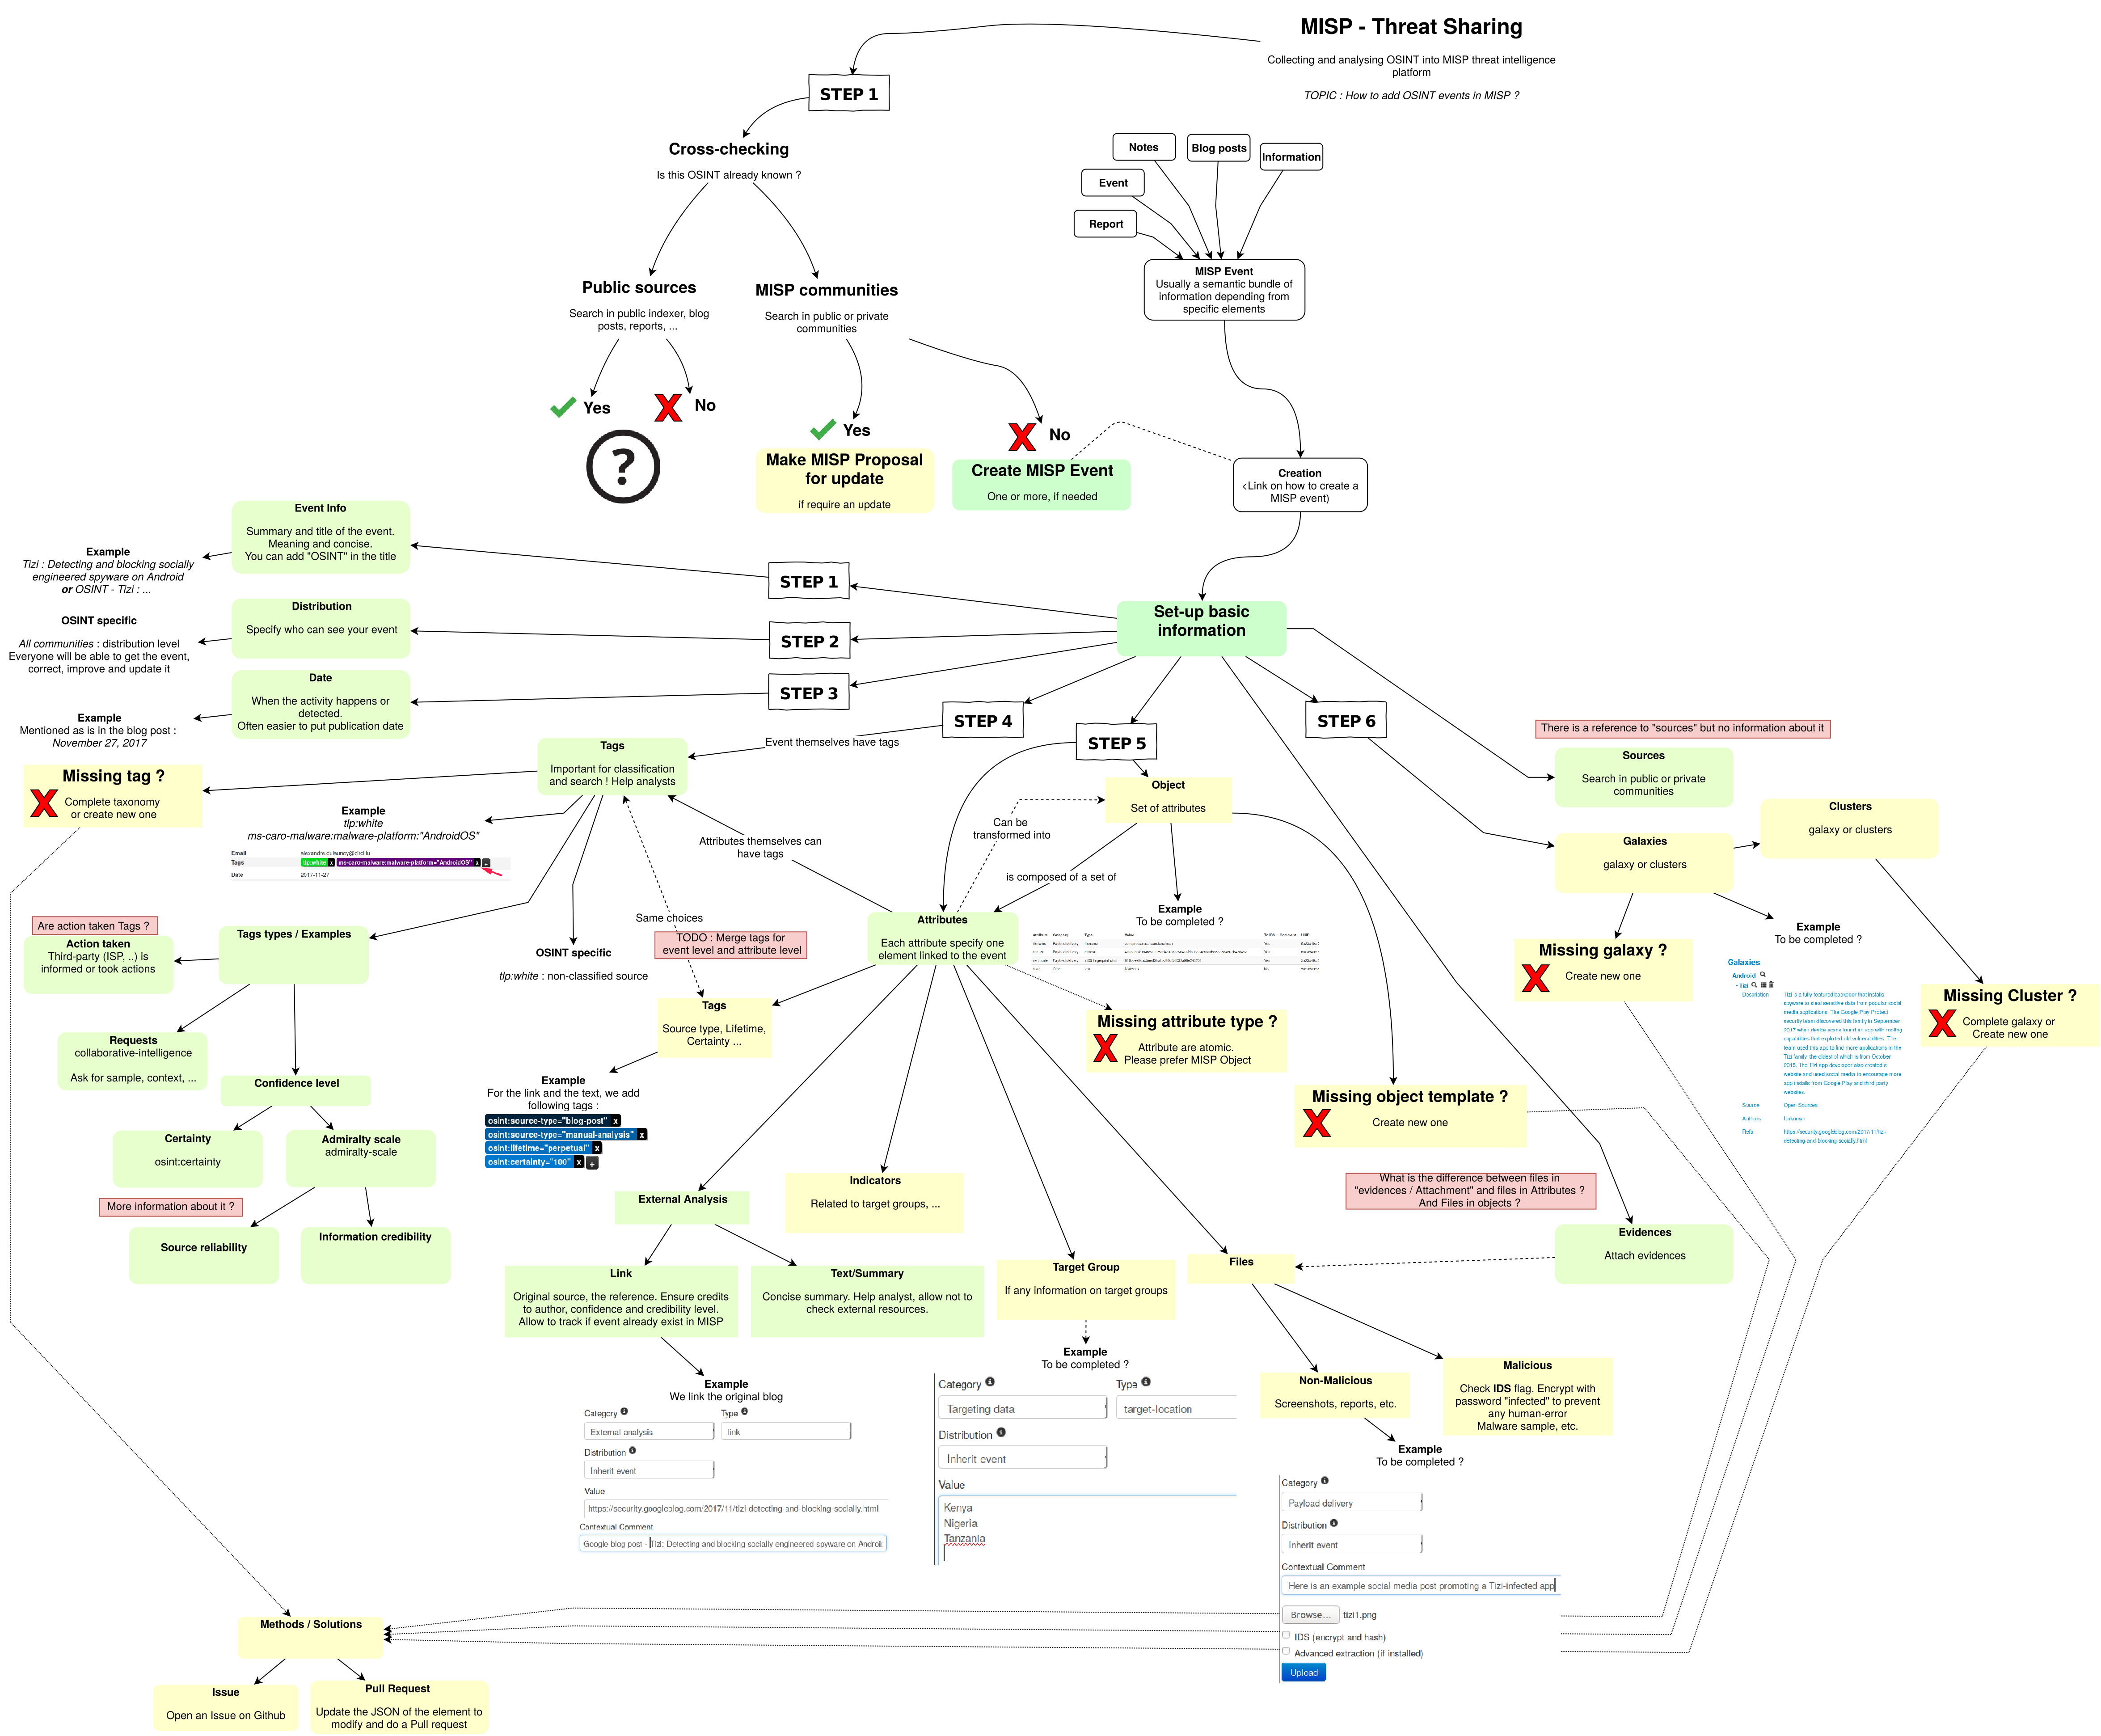
\includegraphics[scale=0.17]{OSINT_MISP_almostcomplete.png}
\end{frame}

\begin{frame}
\frametitle{Meta information and contextualisation 1/2}
\begin{itemize}
\item Quality of indicators/attributes are important but {\bf tagging and classification are also critical to ensure actionable information}
        \item Organizing intelligence is done in MISP by using tags, which often originate from MISP taxonomy libraries
        \item The scope can be classification ({\it tlp, PAP}), type ({\it osint, type, veris}), state ({\it workflow}), collaboration ({\it collaborative-intelligence}), or many other fields
        \item MISP taxonomy documentation is readily available\footnote{\url{https://www.misp-project.org/taxonomies.html}}
        \item {\bf Review existing practices of tagging in your sharing community, reuse practices, and improve context}
\end{itemize}
\end{frame}

\begin{frame}
\frametitle{Meta information and contextualisation 2/2}
\begin{itemize}
        \item {\bf When information cannot be expressed in triple tags format} ({\it namespace:predicate=value}), MISP use Galaxies
        \item {\bf Galaxies} contain a huge set of common libraries\footnote{\url{https://www.misp-project.org/galaxy.html}} such as threat actors, malicious tools, tactics, target information, mitigations, and more
        \item When tagging or adding a Galaxy cluster, tagging at the event level is for the whole event (including attributes and objects). Tagging at the attribute level is for a more specific context
\end{itemize}
\end{frame}

\begin{frame}
        \frametitle{Estimative Probability}
\begin{itemize}
        \item {\bf Words of Estimative Probability}\footnote{\url{https://www.cia.gov/library/center-for-the-study-of-intelligence/csi-publications/books-and-monographs/sherman-kent-and-the-board-of-national-estimates-collected-essays/6words.html}} propose clear wording while estimating probability of occurence from an event
        \item A MISP taxonomy called {\bf estimative-language}\footnote{\url{https://www.misp-project.org/taxonomies.html}} proposes an applied model to tag information in accordance with the concepts of Estimative Probability
\end{itemize}
\end{frame}

\begin{frame}
        \frametitle{Reliability, credibility, and confidence}
\begin{itemize}
        \item The {\bf Admiralty Scale}\footnote{\url{https://www.ijlter.org/index.php/ijlter/article/download/494/234}, {\it US Army Field Manual 2-22.3, 2006}} (also called the {\bf NATO System}) is used to rank the reliability of a source and the credibility of information
        \item A MISP taxonomy called admiralty-scale\footnote{\url{https://www.misp-project.org/taxonomies.html}} is available
        \item US DoD {\bf JP 2-0, Joint Intelligence}\footnote{\url{http://www.jcs.mil/Portals/36/Documents/Doctrine/pubs/jp2\_0.pdf}, page 114} includes an appendix to express confidence in analytic judgments
        \item A MISP predicate in estimative-language called confidence-in-analytic-judgment\footnote{\url{https://www.misp-project.org/taxonomies.html}} is available
\end{itemize}
\end{frame}


\begin{frame}
\frametitle{Adding attributes/objects to an event}
\begin{itemize}
        \item If the information is a {\bf single atomic element}, using a single attribute is preferred
                \begin{itemize}
                        \item Choosing an attribute type is critical as this defines the automation/export rule (e.g. {\it url} versus {\it link} or ip-src/ip-dst?)
                        \item Enabling the IDS (automation) flag is also important, but {\it when you are in doubt}, don't set the IDS flag
                \end{itemize}
        \item If the information is {\bf composite} (ip/port, filename/hash, bank account/BIC), using an object is strongly recommended
\end{itemize}
\end{frame}

\begin{frame}
       \frametitle{How to select the right object?}

        There are more than 150 MISP object\footnote{\url{https://www.misp-project.org/objects.html}} templates.\\
      As an example, at CIRCL, we regularly use the following object templates {\it file}, {\it microblog}, {\it domain-ip}, {\it ip-port}, {\it coin-address}, {\it virustotal-report}, {\it paste}, {\it person}, {\it ail-leak}, {\it pe}, {\it pe-section}, {\it registry-key}.\\
\end{frame}

\begin{frame}
\frametitle{microblog object}
\begin{columns}[totalwidth=\textwidth]
        \column{0.49\textwidth}\underline{Use case}\\
A series of OSINT tweets from a security researcher.
To structure the thread, the information,
and keep a history.\\
        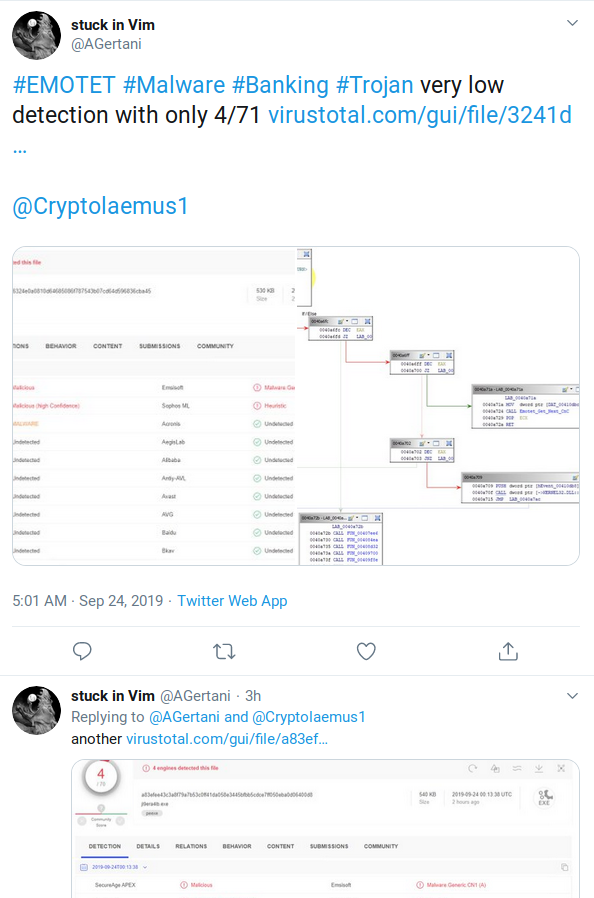
\includegraphics[scale=0.15]{emotet.png}
        \column{0.49\textwidth}\underline{Object to use}\\
        The microblog object can be used for Tweets or any microblog post (e.g. Facebook). The object can be linked using {\it followed-by} to describe a series of post.\\
        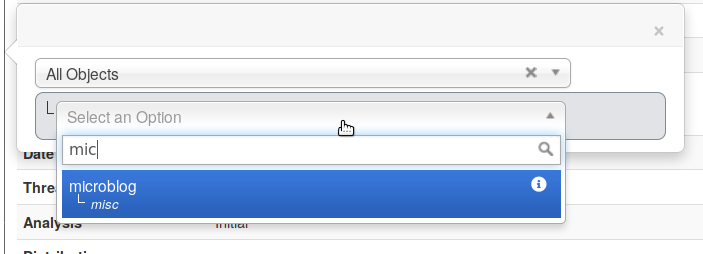
\includegraphics[scale=0.15]{microblog.png}
\end{columns}
\end{frame}


\begin{frame}
\frametitle{file object}
\begin{columns}[totalwidth=\textwidth]
        \column{0.49\textwidth}\underline{Use case}\\
        \begin{itemize}
                \item A file sample was received by email or extracted from VirusTotal
                \item A list of file hashes were included in a report
                \item A hash value was mentioned in a blog post
        \end{itemize}
        \column{0.49\textwidth}\underline{Object to use}\\
        The file object can be used to describe file. It's usual to have partial meta information such as a single hash and a filename.\\
        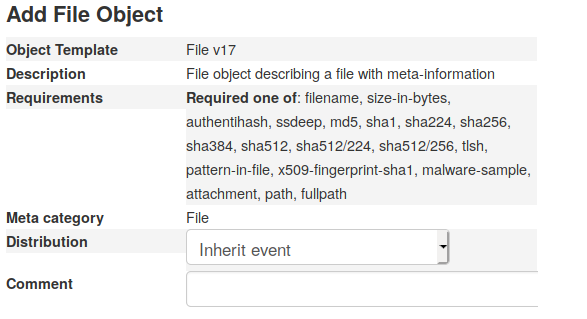
\includegraphics[scale=0.25]{fileobject.png}
\end{columns}
\end{frame}

\begin{frame}
        \frametitle{References}
        \begin{itemize}
        \item Graphical overview of OSINT collection using MISP \url{https://github.com/adulau/misp-osint-collection}
        \item MISP objects documentation \url{https://www.misp-project.org/objects.html}
        \item MISP taxonomies documentation \url{https://www.misp-project.org/taxonomies.html}
        \item MISP galaxy documentation \url{https://www.misp-project.org/galaxy.html}
        \end{itemize}
\end{frame}

